\documentclass{beamer}
\usepackage{graphicx}
\usepackage{amssymb,amsfonts,amsmath}
% \usepackage{tikz,tkz-euclide}
% \usepackage{subfigure}
% \usepackage{parskip}
% \usetikzlibrary{arrows.meta}
% \usetikzlibrary{calc,patterns}
\usefonttheme[onlymath]{serif}
% \usetheme{Berlin}
\title{Weekly Report}
\author{WU Zihan}
\begin{document}
\maketitle
\begin{frame}
    \frametitle{Catalogue}
    \tableofcontents
\end{frame}

\section{Introduction}
\begin{frame}
    \frametitle{Introduction}
    \begin{itemize}
        \item The main task of this week is to run cocluster on the $n$-gram matrix.
        \item After getting the access to fat-node of HPC from CityU, currently the biggest problem is the running time.
        \item Some local running results are shown in the following slides.
    \end{itemize}
\end{frame}

\section{Method}
\begin{frame}
    \frametitle{Method}
    \begin{itemize}
        \item $A\in \mathbb{R}^{27651263\times16094862}$ is the $3$-gram matrix, where we have $27651263$ paragraphs and $16094862$ $3$-grams.
        \item Locally, we select $10000$ paragraphs and all $3$-grams to run cocluster.
        
    \end{itemize}
\end{frame}
\begin{frame}
    \frametitle{Attempt 1}
    \begin{itemize}
        \item First, all zero columns are removed. Then $A \in \mathbb{R}^{10000\times 79728}$.
        % include the figure 'pic/A.png'
        \item Try to do cocluster on $A$ since the linear patterns are emerging.
        \item 
    \end{itemize}
    \begin{figure}[htbp]
        \centering
        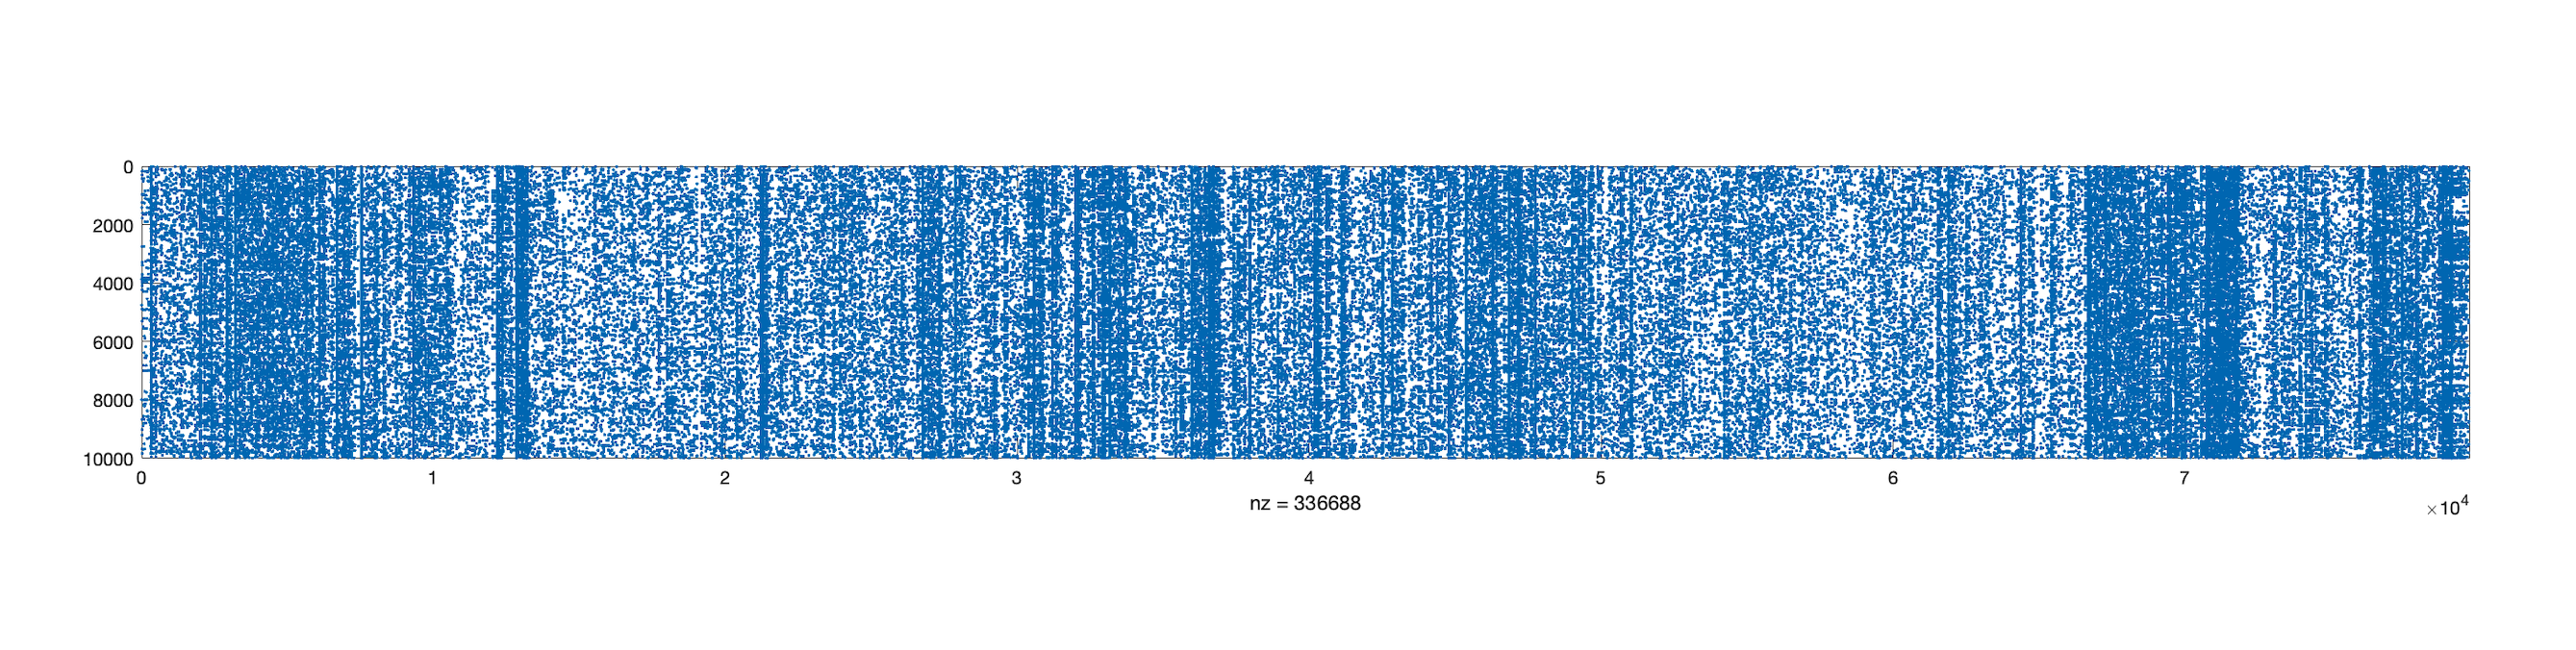
\includegraphics[width=\textwidth]{pic/A.png}
        \caption{The $3$-gram matrix $A$}
    \end{figure}


\end{frame}

\end{document}